\documentclass[11pt]{article}
% Shared preamble for the expert and beginner reports.
\usepackage[T1]{fontenc}
\usepackage[utf8]{inputenc}
\usepackage{lmodern}
\usepackage{microtype}
\DisableLigatures{encoding = T1, family = tt*}  % keep -- as two hyphens in code
\usepackage[a4paper,margin=2.3cm]{geometry}
\usepackage{amsmath,amssymb}
\usepackage{graphicx}
\usepackage{booktabs,longtable,multirow,makecell}
\usepackage{float}
\usepackage{caption}
\usepackage{subcaption}
\usepackage{enumitem}
\usepackage{xcolor}
\usepackage{tikz}
\usetikzlibrary{arrows.meta,positioning,shapes.geometric,calc,decorations.pathreplacing}
\usepackage{algorithm}
\usepackage{algpseudocode}
\usepackage{listings}
\usepackage[most]{tcolorbox}
\usepackage{fancyhdr}
\usepackage[hidelinks]{hyperref}

\graphicspath{{../figures/}}
\setlength{\parskip}{0.45em}
\setlength{\parindent}{0pt}
\setlength{\emergencystretch}{3em}  % long code identifiers: loosen lines instead of overflowing
\setlist{itemsep=0.15em,topsep=0.3em}
\renewcommand{\arraystretch}{1.15}

\definecolor{codebg}{RGB}{246,246,248}
\definecolor{codekw}{RGB}{0,72,150}
\definecolor{codecm}{RGB}{110,110,110}
\definecolor{codestr}{RGB}{140,40,20}
\definecolor{warn}{RGB}{176,64,0}
\definecolor{okc}{RGB}{0,110,60}
\definecolor{boxblue}{RGB}{225,236,250}
\definecolor{boxamber}{RGB}{253,240,215}
\definecolor{boxgreen}{RGB}{226,244,230}
\definecolor{boxgray}{RGB}{238,238,238}

\lstdefinestyle{py}{language=Python,basicstyle=\ttfamily\footnotesize,keywordstyle=\color{codekw}\bfseries,
  commentstyle=\color{codecm}\itshape,stringstyle=\color{codestr},backgroundcolor=\color{codebg},
  frame=single,rulecolor=\color{gray!40},breaklines=true,breakatwhitespace=false,columns=fullflexible,
  keepspaces=true,showstringspaces=false,xleftmargin=0.5em,xrightmargin=0.5em,aboveskip=0.6em,belowskip=0.6em}
\lstdefinestyle{sh}{basicstyle=\ttfamily\footnotesize,backgroundcolor=\color{codebg},frame=single,
  rulecolor=\color{gray!40},breaklines=true,columns=fullflexible,keepspaces=true,showstringspaces=false,
  xleftmargin=0.5em,xrightmargin=0.5em,aboveskip=0.6em,belowskip=0.6em}
\lstset{style=py}

\newtcolorbox{keybox}[1][]{colback=boxblue,colframe=codekw!70,boxrule=0.5pt,arc=2pt,left=6pt,right=6pt,top=4pt,bottom=4pt,fonttitle=\bfseries,#1}
\newtcolorbox{warnbox}[1][]{colback=boxamber,colframe=warn,boxrule=0.5pt,arc=2pt,left=6pt,right=6pt,top=4pt,bottom=4pt,fonttitle=\bfseries,#1}
\newtcolorbox{okbox}[1][]{colback=boxgreen,colframe=okc,boxrule=0.5pt,arc=2pt,left=6pt,right=6pt,top=4pt,bottom=4pt,fonttitle=\bfseries,#1}
\newtcolorbox{notebox}[1][]{colback=boxgray,colframe=gray!60,boxrule=0.5pt,arc=2pt,left=6pt,right=6pt,top=4pt,bottom=4pt,fonttitle=\bfseries,#1}

% Notation
\newcommand{\kT}{k_{\mathrm{B}}T}
\newcommand{\xiP}{\xi_{P}}
\newcommand{\gl}{\gamma_{l}}
\newcommand{\Pe}{\mathrm{Pe}}
\newcommand{\Flex}{\mathfrak{F}}
\newcommand{\spn}{\mathfrak{s}}
\newcommand{\dd}{\mathrm{d}}
\newcommand{\vect}[1]{\mathbf{#1}}
\newcommand{\code}[1]{\texttt{\detokenize{#1}}}
\newcommand{\NR}{\textbf{not a replication}}

\pagestyle{fancy}
\fancyhf{}
\renewcommand{\headrulewidth}{0.3pt}
\fancyfoot[C]{\thepage}

\fancyhead[L]{\small Self-propelled filaments that wind into spirals}
\fancyhead[R]{\small Learning report}

\title{\textbf{How a Self-Propelled Filament Winds Itself into a Spiral}\\[0.4em]
\large A from-scratch guide to our reproduction of Isele-Holder, Elgeti \& Gompper (2015):\\
the physics, the simulation, the measurements, the code, and what we found\\[0.5em]
\normalsize Learning report (for newcomers)}
\author{Prepared with Claude Code for the spin-chain-polymer project}
\date{5 October 2026}

\begin{document}
\maketitle
\thispagestyle{empty}

\begin{keybox}[title=What this document is]
This is a teaching version of our technical report. It assumes you know some high-school physics and a little programming, and nothing else.
Every idea is built up from scratch: why tiny things jiggle, what a ``Péclet number'' is, how a computer moves beads forward in time,
how we measure a spiral, how we made sure the computer was not fooling us, and how to run the code yourself.
At the end there is a glossary and a set of exercises with answers. A companion \emph{expert report} has the same facts in compressed form.
\end{keybox}

\begin{notebox}[title=The one-paragraph story]
A 2015 paper showed, by computer simulation, that a flexible filament pushed along its own length (like a self-driving worm on a surface) can bump into itself with its head and
wind up into a stable spiral. We set out to reproduce that study carefully. We checked the physics equations against two copies of the paper, found and fixed a hidden bug that
had been quietly moving every saved snapshot back to the origin, built tools to measure everything the paper measures, and tested each tool on cases where we know the right answer.
We then ran one long simulation, more than two days of computer time, at the paper's ``strong spiral'' setting. The filament spent \textbf{97.8\%} of its time wound into a spiral,
including one spiral that lasted for over 2000 body-lengths of travel. That agrees with the paper, \emph{for this one run}. It is not yet a full reproduction, because one run on one random seed cannot tell us how typical it is, and two settings the
authors used were never published.
\end{notebox}

\tableofcontents
\newpage

%=====================================================================
\section{The physics you need, from zero}
%=====================================================================
\subsection{What is being simulated?}
Picture a thin, bendy thread lying flat on a surface: a protein filament on a glass slide, or a long thin bacterium. We model it as a necklace of beads joined by springs,
the \emph{bead--spring model}. Here it has $N+1=101$ beads and $N=100$ springs (bonds). Each bead is pushed forward along the thread's own direction,
like tiny motors underneath it. Figure~\ref{fig:beads} shows the idea.

\begin{figure}[H]\centering
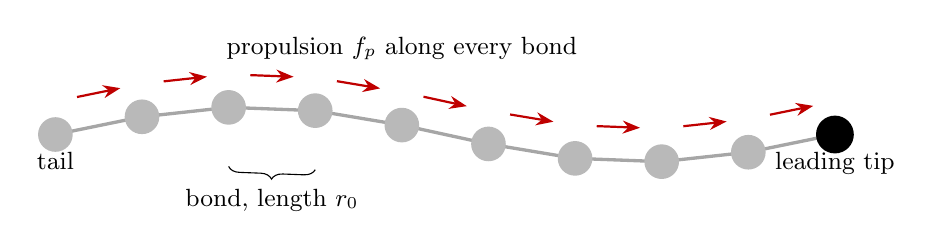
\begin{tikzpicture}[scale=1.0]
\foreach \i in {0,...,9}{ \pgfmathsetmacro{\x}{1.1*\i} \pgfmathsetmacro{\y}{0.35*sin(40*\i)}
  \coordinate (b\i) at (\x,\y); }
\foreach \i [count=\j from 1] in {0,...,8}{ \draw[gray!70,line width=1.2pt] (b\i) -- (b\j); }
\foreach \i in {0,...,8}{ \fill[gray!55] (b\i) circle (0.22); }
\fill[black] (b9) circle (0.24);
\foreach \i [count=\j from 1] in {0,...,8}{ \draw[-{Stealth[length=2.2mm]},red!75!black,thick] ($(b\i)!0.25!(b\j)+(0,0.42)$) -- ($(b\i)!0.75!(b\j)+(0,0.42)$); }
\node[above] at ($(b4)+(0,0.7)$) {\small propulsion $f_p$ along every bond};
\node[below=3pt] at (b9) {\small leading tip};
\node[below=3pt] at (b0) {\small tail};
\draw[decorate,decoration={brace,amplitude=4pt,mirror}] ($(b2)+(0,-0.75)$) -- ($(b3)+(0,-0.75)$) node[midway,below=4pt]{\small bond, length $r_0$};
\end{tikzpicture}
\caption{The bead--spring filament. Grey beads are joined by stiff springs; every bond is pushed along its own direction (red arrows), so the whole chain crawls along its contour. The black bead is the leading tip.}
\label{fig:beads}
\end{figure}

\subsection{Why tiny things jiggle: thermal noise and $\kT$}
Molecules of the surrounding liquid hit the filament billions of times per second from random directions. The net effect is a random, ever-changing push: \emph{Brownian motion}.
Its strength is set by temperature through the energy scale $\kT$ (Boltzmann's constant times temperature). In our simulation everything is measured in units where $\kT=1$.

A free particle doing Brownian motion wanders away from its start, but not in a straight line. Its \emph{mean square displacement} (MSD) grows in proportion to time,
$\langle\Delta r^2\rangle=4Dt$ in two dimensions, where $D$ is the diffusion coefficient. A particle moving at constant velocity has instead $\langle\Delta r^2\rangle=v^2t^2$.
On a log--log plot, diffusion has slope~1 and straight-line (\emph{ballistic}) motion has slope~2. We use this slope trick many times.

\subsection{No inertia: the overdamped world}
For something micrometres long in water, friction is enormous compared with inertia: stop pushing, and it stops almost instantly, like a spoon in honey.
So instead of Newton's ``force = mass $\times$ acceleration'' we use \emph{force = friction $\times$ velocity}:
\begin{equation}
\gamma\,\dot{\vect r}_i = \text{(spring and bending forces)} + \text{(random thermal force)} + \text{(propulsion)} .
\end{equation}
Here $\gamma$ is the friction coefficient of one bead. This is called \emph{overdamped} or \emph{Brownian} dynamics, and it is what the paper's Eq.~1 says.

\subsection{Stiffness and the persistence length}
A filament resists bending. We measure stiffness with the \emph{persistence length} $\xiP$: roughly, how far along the filament you must go before it ``forgets'' which way it was pointing.
A dry spaghetti strand has a huge persistence length; cooked spaghetti a short one. The paper uses the ratio $\xiP/L$, persistence length divided by total length $L$.
We focus on $\xiP/L=0.2$: the filament is five persistence lengths long, so it is quite floppy.

\begin{keybox}[title=Why the factor $1/4$ in the bending energy matters]
The paper writes the bending energy as $\frac{\kappa}{4}\sum(\text{difference of neighbouring bond vectors})^2$. For small angles $\theta$ between neighbouring bonds this is
$\frac{\kappa}{4}\theta^2$ per joint. Thermal physics then gives an average $\langle\theta^2\rangle=2\kT/\kappa$, and the direction memory decays like $e^{-s\,\kT/\kappa}$ along the chain.
So the persistence length is exactly $\xiP=\kappa/\kT$, which is the paper's Eq.~8. Drop the $1/4$ and the filament becomes four times stiffer than intended.
That is why the rules said: never touch the $1/4$.
\end{keybox}

\subsection{Active matter: pushing along your own length}
Ordinary filaments only jiggle. \emph{Active} filaments burn energy to move by themselves. Here every bond is pushed along its own direction with force $f_p$ per unit length.
Because the push always follows the chain's own shape, the chain slides along its own outline, like a train following its tracks. The paper calls this \emph{railway motion}.

\subsection{No crossing: excluded volume}
Two parts of the filament cannot pass through each other. This is enforced by a short-range repulsion between beads (the WCA potential). It is zero beyond a distance of about 1.12 bead diameters and very steep closer than that.
This rule is what makes spirals possible: when the head bumps into the body, it cannot pass through, so it is forced to turn.

\subsection{The three numbers that control everything}
Physicists like \emph{dimensionless numbers}: ratios that say which effect wins. The paper uses three.
\begin{itemize}
\item \textbf{Stiffness} $\xiP/L=\kappa/(\kT L)$: small means floppy.
\item \textbf{Péclet number} $\Pe=f_pL^2/\kT$: directed motion versus random jiggling. $\Pe=200$ is weakly pushed; $\Pe=5000$ is strongly pushed.
\item \textbf{Flexure number} $\Flex=\Pe/(\xiP/L)=f_pL^3/\kappa$: pushing versus stiffness. Large $\Flex$ means a strong push on a floppy filament, which favours spirals.
\end{itemize}
And two clocks:
\begin{itemize}
\item $\tau=L^3\gl/(4\kT)$, the time to diffuse one body length. With our units $\tau=252\,500$ time units. The paper ran ``more than $5\tau$''.
\item The \textbf{contour time} $t_c=L\gl/f_p$, the time to crawl one body length. At $\Pe=5000$, $t_c=202$ time units, so $5\tau$ is \textbf{6250 contour lengths} of crawling.
\end{itemize}
($\gl=\gamma(N+1)/L$ is the friction per unit length; with our numbers $\gl=1.01$.)

\begin{notebox}[title=Worked example: from Pe to forces]
With $L=100$ and $\kT=1$: $f_p=\Pe/L^2$. So $\Pe=5000$ gives $f_p=0.5$. Bending stiffness $\kappa=(\xiP/L)\,\kT L=0.2\times100=20$. The flexure number is $\Flex=5000/0.2=25\,000$.
The crawl speed is $v_c=f_p/\gl=0.5/1.01\approx0.495$ bead-lengths per time unit.
\end{notebox}

\subsection{How a spiral forms and breaks}
\begin{figure}[H]\centering
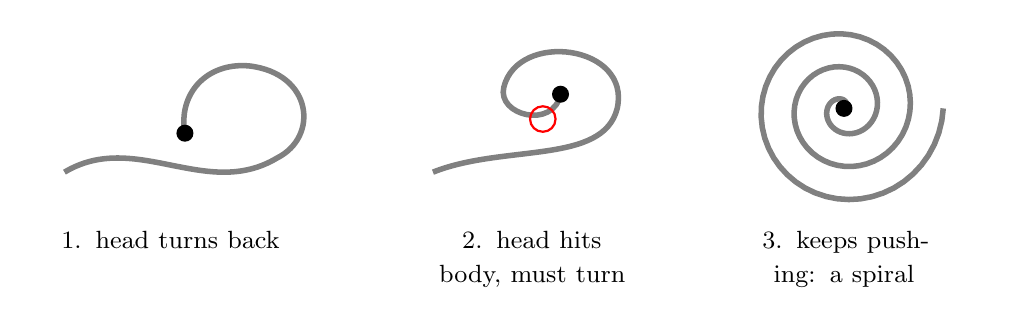
\begin{tikzpicture}[scale=0.9]
\begin{scope}
\draw[gray,line width=2pt] (0,0) .. controls (1,0.6) and (2,-0.4) .. (3,0.2) .. controls (3.6,0.5) and (3.5,1.4) .. (2.6,1.5) .. controls (2.0,1.55) and (1.6,1.1) .. (1.7,0.55);
\fill (1.7,0.55) circle (0.12); \node[below,text width=3.4cm,align=center] at (1.5,-0.7) {\small 1. head turns back};
\end{scope}
\begin{scope}[xshift=5.2cm]
\draw[gray,line width=2pt] (0,0) .. controls (1,0.4) and (2.4,0.1) .. (2.6,0.9) .. controls (2.8,1.8) and (1.2,2.0) .. (1.0,1.2) .. controls (0.9,0.8) and (1.7,0.6) .. (1.8,1.1);
\fill (1.8,1.1) circle (0.12); \draw[red,thick] (1.55,0.75) circle (0.18); \node[below,text width=3.4cm,align=center] at (1.4,-0.7) {\small 2. head hits body, must turn};
\end{scope}
\begin{scope}[xshift=11cm,yshift=0.9cm]
\draw[gray,line width=2pt,domain=0:1080,samples=150,variable=\t] plot ({0.0013*\t*cos(\t)},{0.0013*\t*sin(\t)});
\fill (0,0) circle (0.12); \node[below,text width=3.4cm,align=center] at (0,-1.6) {\small 3. keeps pushing: a spiral};
\end{scope}
\end{tikzpicture}
\caption{Spiral formation (cartoon of the paper's Fig.~3a). The leading tip (black) collides with the body, excluded volume forces it to bend, and continued propulsion winds the chain up with the tip in the centre.}
\label{fig:formation}
\end{figure}
Once wound, the spiral spins in place: the propulsion now drives rotation instead of travel. It breaks up in one of two ways. The tip can spontaneously change direction
(thermally activated, most likely in floppy filaments), or bending stiffness can slowly unwind the spiral until the tip loses contact (widening, in stiffer filaments;
the paper finds this happens when $\Flex\lesssim1000$--$1500$). Our setting has $\Flex=25\,000$, so we expect the first kind.

The paper names three \textbf{regimes}:
\begin{itemize}
\item \emph{polymer}: no spirals, $\Pe=200$;
\item \emph{weak spiral}: occasional short-lived spirals, $\Pe=1000$;
\item \emph{strong spiral}: spirals dominate, $\Pe=5000$.
\end{itemize}
These are the three panels of its Figure~2.

%=====================================================================
\section{The model, term by term}
%=====================================================================
For readers ready for the full equations, here they are with a plain-language reading. $\vect r_i$ is the position of bead $i$; $\vect r_{i,j}=\vect r_i-\vect r_j$.
\begin{center}\small
\begin{tabular}{p{0.44\linewidth}p{0.48\linewidth}}\toprule equation & what it says\\ \midrule
$U_\mathrm{bond}=\frac{k_S}{2}\sum(|\vect r_{i,i+1}|-r_0)^2$ & bonds are stiff springs of rest length $r_0$ ($k_S=4000\,\kT/r_0^2$) \\
$U_\mathrm{angle}=\frac{\kappa}{4}\sum(\vect r_{i,i+1}-\vect r_{i+1,i+2})^2$ & bending costs energy; straight is cheapest \\
$u_\mathrm{EV}(r)=4\epsilon[(\sigma/r)^{12}-(\sigma/r)^{6}]+\epsilon$ for $r<2^{1/6}\sigma$ & beads closer than about $1.12\sigma$ repel strongly; further apart, nothing \\
$\vect F_p=\sum f_p\,\vect r_{i,i+1}$, split equally on both beads & every bond is pushed along itself \\
$\gamma\dot{\vect r}_i=-\nabla_iU+\vect F^{(i)}_{\kT}+\vect F^{(i)}_p$ & friction balances all forces (overdamped) \\ \bottomrule
\end{tabular}
\end{center}
Settings: $r_0=\sigma=1$ (bead size equals bond length), $\epsilon=\kT=1$, $\gamma=1$.

\begin{warnbox}[title=Two numbers we do not have]
The paper says its timestep $\Delta t$ ``was adjusted'' for each run and lists the values in a supplementary file (the ESI). It also used a modified version of the LAMMPS simulation package, whose input files
decide exactly which nearby bead pairs feel the repulsion. Neither the timestep table nor that setting is in the paper or its arXiv source. We used a safe timestep of our own,
and we keep the question of which bead pairs repel (the ``exclusion policy'') open. Both are labelled clearly everywhere.
\end{warnbox}

%=====================================================================
\section{Teaching a computer to move the beads}
%=====================================================================
\subsection{Small steps in time: Euler--Maruyama}
A computer cannot follow continuous time; it takes small steps $\Delta t$. For overdamped motion with noise, the simplest correct recipe is the
\emph{Euler--Maruyama} step:
\begin{equation}
\vect r_i^{\,\mathrm{new}}=\vect r_i+\underbrace{\frac{\Delta t}{\gamma}\vect F_i}_{\text{drift from forces}}+\underbrace{\sqrt{\frac{2\kT\Delta t}{\gamma}}\,\boldsymbol\xi_i}_{\text{random kick}},\qquad \boldsymbol\xi_i=\text{two standard normal random numbers}.
\end{equation}
Notice the kick scales like $\sqrt{\Delta t}$, not $\Delta t$. That is the signature of diffusion: after $n$ steps random kicks add up like a random walk, to about $\sqrt{n}$ times one kick.

\begin{notebox}[title=Worked example: one free bead]
With $\kT=\gamma=1$ and $\Delta t=5\times10^{-5}$, each kick has size $\sqrt{2\times5\times10^{-5}}=0.01$ per direction. After $10^6$ steps ($t=50$),
the expected squared distance is $4Dt=4\times1\times50=200$, about 14 bead lengths. Equivalently, each kick has variance $2\kT\Delta t/\gamma=10^{-4}$ in each of 2 directions, and $10^6$ of them sum to $2\times10^6\times10^{-4}=200$. The two pictures agree.
\end{notebox}

\subsection{Why the timestep must be tiny}
The bond springs are very stiff ($k_S=4000$). A spring relaxes in about $\gamma/k_S=2.5\times10^{-4}$ time units. If a step is longer than that, the update overshoots and the simulation explodes.
The code refuses any $\Delta t$ above $0.2\gamma/k_S=5\times10^{-5}$, and we use exactly that value. The consequence is that $5\tau$ needs $252\,500\times5/(5\times10^{-5})=\mathbf{2.525\times10^{10}}$ \textbf{steps}.
At about 120\,000 steps per second, that is roughly 2.4 days for one run.

\subsection{Random numbers you can replay}
A simulation needs billions of random numbers. Our generator is special: the numbers for ``seed $S$, step $t$, bead $i$'' are computed directly from those three integers,
like looking up a page in a book rather than reading a story from the beginning. It uses a scrambling function called SplitMix64 and the Box--Muller formula to turn uniform numbers into Gaussian ones.
The payoff is \textbf{replayability}. Stop a run, restart it tomorrow, or split it into pieces, and you get bit-for-bit the same trajectory. We test this.

\subsection{Not checking every pair: neighbour lists}
Excluded volume needs the distance between pairs of beads. There are about 5000 pairs, but at any moment only a handful are close. A \emph{Verlet neighbour list} records the pairs closer than the
cutoff plus a safety margin (the \emph{skin}, 0.4). The list is rebuilt only when some bead has moved more than half the skin. As long as nobody has moved that far, no pair outside the list can
have come within the cutoff, so the shortcut gives \emph{exactly} the same forces as checking all pairs. It is a pure speedup.

\begin{algorithm}[H]
\caption{One simulation step (simplified)}
\begin{algorithmic}[1]
\If{any bead moved more than skin/2 since the last list} rebuild the neighbour list \EndIf
\State compute spring, bending and propulsion forces along the chain
\State add repulsion for listed pairs that are actually closer than the cutoff
\For{each bead $i$}
  \State draw two Gaussian numbers from (seed, step, $i$)
  \State move bead: drift $\frac{\Delta t}{\gamma}\vect F_i$ plus kick $\sqrt{2\kT\Delta t/\gamma}\,\boldsymbol\xi_i$
\EndFor
\end{algorithmic}
\end{algorithm}

%=====================================================================
\section{Measuring what the filament does}
%=====================================================================
\subsection{The spiral number $\spn$}
Walk along the filament from tail to tip and add up how much the direction turns (left turns positive, right turns negative). Divide the total by a full turn ($2\pi$). That number is $\spn$.
\begin{itemize}
\item A straight filament: no turning, $\spn=0$.
\item A filament bent into a full circle: one turn, $\spn=\pm1$.
\item A spiral with four windings: $\spn\approx\pm4$.
\end{itemize}
The sign only says clockwise or anticlockwise, so we usually look at $|\spn|$. Our spirals sit at $|\spn|\approx4$.

\subsection{Histograms and the kurtosis $\beta_2$}
Record $\spn$ many times and draw a histogram of $|\spn|$. The \emph{kurtosis} $\beta_2$ is a single number describing the histogram's shape: the average of (distance from the mean)$^4$
divided by (variance)$^2$. Following the paper, we count every $|\spn|$ twice, once as $+|\spn|$ and once as $-|\spn|$, to make the distribution symmetric.

\begin{notebox}[title=Worked examples of $\beta_2$]
\begin{itemize}
\item A bell curve (Gaussian) has $\beta_2=3$: this is the polymer regime, with $\spn$ wobbling around 0.
\item All values exactly at $\pm4$: deviations are all $4$, so $\beta_2=4^4/(4^2)^2=1$. This is the strong-spiral regime: two sharp peaks.
\item Mostly near 0 with rare excursions to $\pm3$: the rare far values inflate the fourth power. $\beta_2>3$: the weak-spiral regime.
\end{itemize}
So $\beta_2$ near 1 means ``nearly always wound''. Our long run gave $\beta_2=1.03$.
\end{notebox}

\subsection{Mean square displacement, again}
For the centre of mass (COM) we compute the MSD at many time lags, averaging over every possible starting time (``multi-origin'' averaging).
We report lags in real time units, never just as ``number of frames''. The log--log slope tells the story: 1 is diffusive, 2 is ballistic.

\subsection{Railway motion (the paper's Figure~6)}\label{sec:b-railway}
Take bead $j$ and a bead $i$ places behind it. If the chain slides along its own track, then after the time needed to crawl $i$ bond lengths, bead $j+i$ sits where bead $j$ was.
Its MSD \emph{relative to bead $j$'s old position} drops to a minimum that touches the ordinary thermal jiggle of a bead in a passive filament. Seeing that dip is the fingerprint of railway motion.

\begin{keybox}[title=Which end is the head? A subtle bookkeeping point]
In the paper the propulsion is written so that \emph{bead~1} leads. In our code the propulsion pushes towards the \emph{last} bead. Physically this is the same filament
with the beads numbered backwards. So we did not change the physics; we translate the numbering: paper bead $k$ is code bead $101-k$, so paper bead 25 is code bead 76.
Getting this wrong would make Figure~6 compare the wrong beads.
\end{keybox}

\subsection{Rotation and its pitfall}
Track the angle of the end-to-end vector (tail to tip), counting full turns, so it can grow past $360^\circ$. Its mean square change (MSR) also has a log--log slope: 2 for steady spinning (a spiral),
and 1 for random reorientation, whose rate is the rotational diffusion coefficient $D_r$. The paper fits $D_r$ only where the slope is 1. A warning from our experience: in short runs the curve can pass
\emph{through} slope 1 on its way from one regime to another. A mechanical rule then ``finds'' a meaningless $D_r$, so always look at the curve.

\subsection{The dynamic structure factor}
$S(q,t)$ asks how similar the filament's shape pattern at one moment is to its pattern a time $t$ later, at a length scale set by $q$ (we use $q=5\pi/L$, about a fifth of the filament).
It decays as the shape changes or the filament moves away. Its typical decay time $\tau_S$ measures how fast the filament explores new shapes. The paper never says over which time range to integrate; we state ours.

%=====================================================================
\section{Making sure the computer is not fooling us}
%=====================================================================
\subsection{Tests: questions with known answers}
A \emph{unit test} runs a small piece of code on a case where we already know the right answer. We have \textbf{64} tests, and all pass. Examples:
\begin{itemize}
\item The forces must equal minus the slope of the energy: we compare against a numerical derivative.
\item On a straight chain, the total propulsion must equal $f_p\times$(tip position $-$ tail position).
\item The spiral number of a drawn three-turn spiral must come out about 3.2.
\item The kurtosis of a bell curve must be 3, and of values at exactly $\pm a$ must be 1.
\item A run stopped and resumed must equal an uninterrupted run, bit for bit.
\end{itemize}
A good test has one clear assertion and checks a \emph{meaning}, not just that ``a number came out''.

\subsection{Detective story: the bug that moved the world back to zero}\label{sec:b-bug}
The original code had a hidden habit. Every 10\,000 steps it shifted the whole filament so its centre of mass sat at the origin, and it did not record how far it had shifted it.
\begin{itemize}
\item \textbf{Harmless for shape.} A spiral looks the same wherever it is.
\item \textbf{Disastrous for motion.} Every saved snapshot had its centre of mass reset to almost exactly zero. The ``distance travelled'' (the paper's Figure~9) and the structure factor (Figure~10), which both compare positions at different times, became meaningless.
\end{itemize}
\textbf{How we caught it.} We first wrote a test that \emph{fails} if a pushed filament's stored centre sits at zero on a reset step. On the original code it failed: the stored value was $2\times10^{-17}$, which is zero to computer precision.
\textbf{How we fixed it.} Shifting is now off on the production path. If anyone switches it on, the code forces them to record the shift. Every file now states its \emph{origin convention}, a single fixed origin for all frames, and older files are refused.
\textbf{Lesson.} Write the test that would catch the bug \emph{before} fixing it, and watch it fail.

\subsection{Saving your game: checkpoints, resume, segments, stitching}
A 2.5-day run must survive interruptions, so the program does four things:
\begin{itemize}
\item \textbf{Checkpoint.} At every saved frame (about every 9 seconds) it writes the exact positions and the step number to a small file. The step number is all it needs to regenerate the random numbers.
\item \textbf{Resume.} After a crash it reloads the checkpoint and continues into a \emph{new} file, called a \emph{segment}, so nothing already saved can be overwritten.
\item \textbf{Stitch.} Afterwards, the segments are joined. The join must match exactly (same positions at the shared moment); gaps or overlaps are refused.
\item \textbf{Flush.} Before every checkpoint, the data file is written to disk, so the checkpoint never refers to unsaved data.
\end{itemize}

\begin{figure}[H]\centering
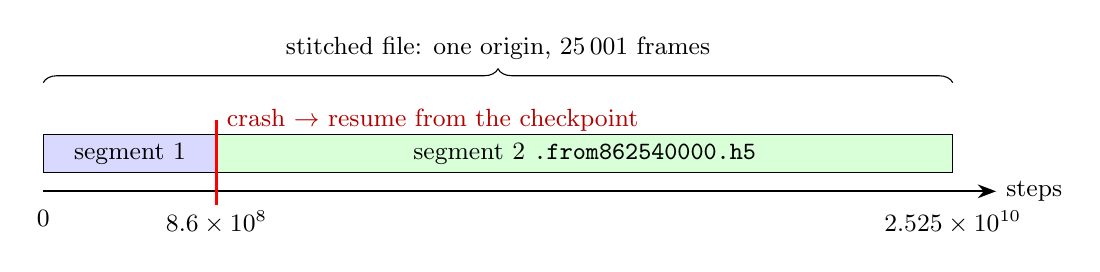
\begin{tikzpicture}[x=0.55cm,y=0.6cm]
\draw[thick,-{Stealth}] (0,0) -- (22,0) node[right]{\small steps};
\draw[fill=blue!15] (0,0.4) rectangle (4,1.2) node[midway]{\small segment 1};
\draw[fill=green!15] (4,0.4) rectangle (21,1.2) node[midway]{\small segment 2 \texttt{.from862540000.h5}};
\draw[red,thick] (4,-0.3) -- (4,1.5) node[right,font=\small,text=red!70!black]{crash $\rightarrow$ resume from the checkpoint};
\node[below] at (0,-0.2) {\small 0}; \node[below] at (4,-0.2) {\small $8.6\times10^8$}; \node[below] at (21,-0.2) {\small $2.525\times10^{10}$};
\draw[decorate,decoration={brace,amplitude=5pt}] (0,2.3) -- (21,2.3) node[midway,above=5pt]{\small stitched file: one origin, 25\,001 frames};
\end{tikzpicture}
\caption{How our long run was saved: two segments joined exactly at the checkpoint step.}
\end{figure}

\subsection{Deciding the rules before looking: the verdict}\label{sec:b-verdict}
It is tempting to look at the data and then pick a definition that makes it look good. To avoid that, we wrote the \emph{verdict} rules before the run finished.
\begin{itemize}
\item Ignore the first $0.5\tau$, the start-up period.
\item Measure: the fraction of time with $|\spn|>2$; $\beta_2$; the longest unbroken stretch (``plateau'') with $|\spn|>2$, in contour lengths; and a few motion slopes.
\item Then apply fixed descriptions:
\begin{itemize}
\item \emph{predominant}: fraction above $1/2$ and $\beta_2<2$;
\item \emph{intermittent}: some plateau longer than 2 contours, but fraction below $1/2$;
\item \emph{absent}: no such plateau.
\end{itemize}
\end{itemize}
The verdict refuses to judge a file shorter than $5\tau$, a file without a stated origin, or a file whose stored centre does not match its stored beads.

%=====================================================================
\section{What we did, in order}
%=====================================================================
The work happened in six sessions. Each one started by checking a fingerprint (a SHA-256 hash) of the code we were handed, so that we never built on the wrong version.

\subsection*{Session 1: audit and repair}
\begin{itemize}
\item \textbf{Checked the physics.} We compared the code's equations against the published PDF and the arXiv \LaTeX{} source. They matched.
Several suspected misprints we had been warned about (a square root in Eq.~3, an extra $L^2$ in Eq.~8, $\Flex=2500$ in a caption) turned out to be artefacts of copying text out of the PDF, not real misprints.
\item \textbf{Found the zero-reset bug} and fixed it, test first (Section~\ref{sec:b-bug}).
\item \textbf{Worked out which end leads} and translated the bead numbering (Section~\ref{sec:b-railway}).
\item \textbf{Built the measuring tools}, each with a test: railway MSD, rotation, structure factor, histogram, plateau finder.
\item \textbf{Ran a smoke test} (a quick ``does it switch on?'' run). Over 4000 steps at $\Pe=200$ the filament's centre moved 0.127 bead lengths and was never reset to zero, and $\spn$ stayed below 0.14.
A longer 2-million-step check at $\Pe=1000$ showed railway motion: the relative-MSD dips appeared near the predicted times (at lag 14.8 for $i=1$, predicted 10; 21.9 for $i=2$, predicted 20; 40.2 for $i=4$, predicted 40).
\end{itemize}

\subsection*{Session 2: pictures}
We built a visualizer: films of the saved snapshots, with no invented in-between frames, plus summary panels. All three Figure-2 settings were run for 100 time units each.
None formed a spiral. That was expected: 100 time units is only half a contour length even at the fastest setting.
\begin{figure}[H]\centering
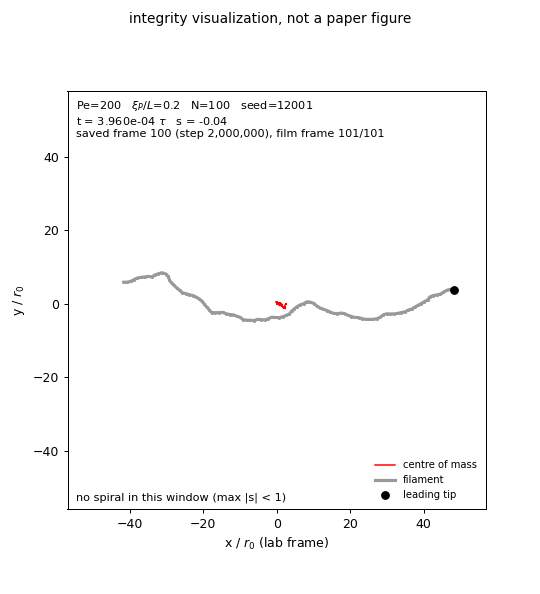
\includegraphics[width=0.38\linewidth]{frame_viz_polymer_last.png}\hspace{1em}
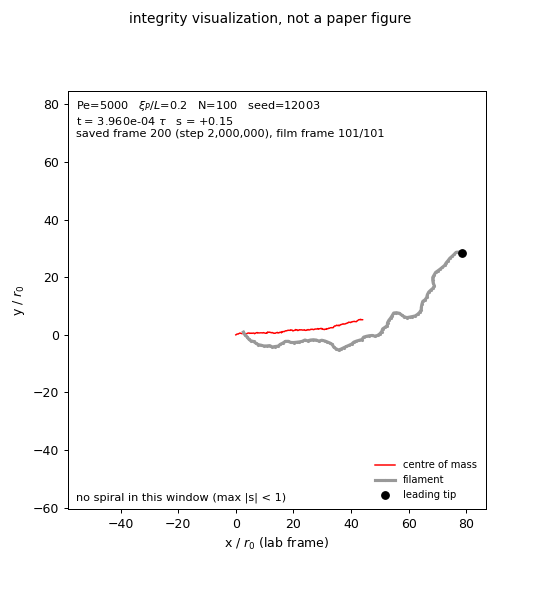
\includegraphics[width=0.38\linewidth]{frame_viz_strong_last.png}
\caption{Last frames of the session-2 films: $\Pe=200$ (left) and $\Pe=5000$ (right) after 100 time units. Grey filament, black head, red centre-of-mass trail. Too short for a spiral.}
\end{figure}

\subsection*{Session 3: the formation test (``gate'') and a mistake}
Before spending days on one long run, we ran a cheap test: does a spiral form within 10 contour lengths (about 5 minutes of computing)?
The pass rule: $|\spn|>2$ held for at least 2 contour lengths, and the centre-of-mass bookkeeping intact.
\begin{itemize}
\item Seed 12013 with the \code{paper_all_pairs} policy passed: a spiral at $\spn\approx-4.1$ for 3.8 contours.
\item Seed 12003 with \code{lammps_default} failed.
\end{itemize}
We then started a long run, but with the \emph{wrong} seed (12003, never shown to spiral under that policy) and with snapshots too far apart (one every 12.5 contours, longer than the whole spiral we had seen). It was stopped and never used.

\subsection*{Session 4: untangling seed from policy}
The first gate changed two things at once, the policy \emph{and} the seed, so we crossed them:
\begin{figure}[H]\centering
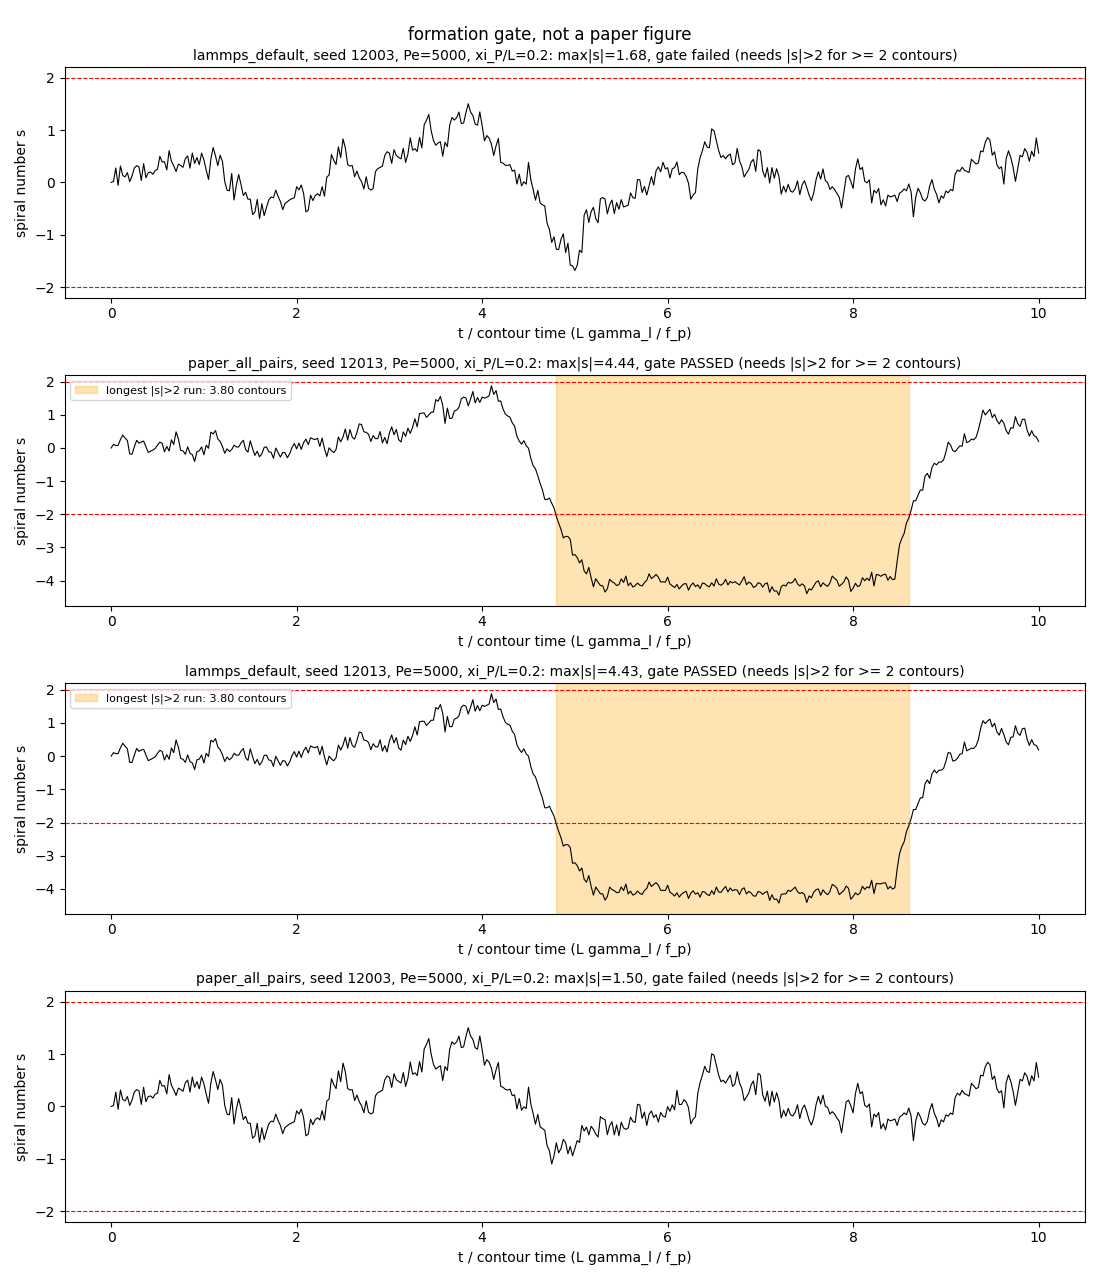
\includegraphics[width=0.78\linewidth]{gate4_s_t.png}
\caption{The four gate runs (10 contours each). Seed 12013 winds up under \emph{both} policies; seed 12003 under \emph{neither}. The random seed decided, not the policy.}
\end{figure}
Why did the seed matter more than the policy? With the same seed, both runs receive identical random kicks. The two policies differ only for beads at most 3 apart along the chain, while
spirals form when beads far apart touch. So the runs stay almost identical. The lesson: change one thing at a time.

We also built the tools for the long run:
\begin{itemize}
\item snapshots every 0.25 contour, so a 3.8-contour spiral spans about 15 frames;
\item a \code{--seed} option;
\item the segment stitcher;
\item a zoomed film of the spiral.
\end{itemize}
\begin{figure}[H]\centering
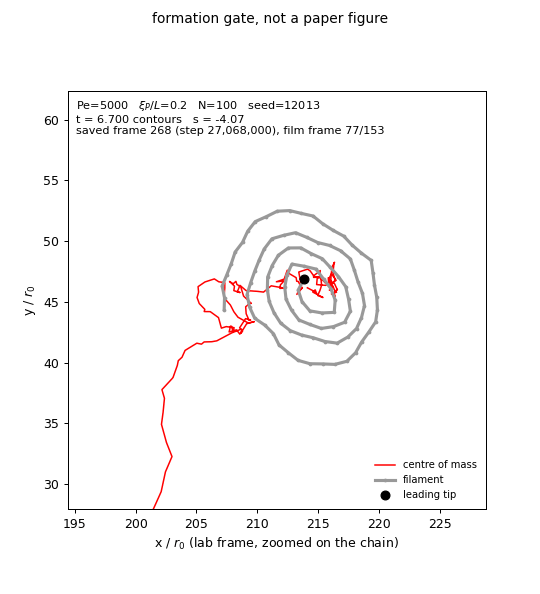
\includegraphics[width=0.42\linewidth]{frame_gate_plateau.png}
\caption{Zoom on the wound filament in the gate run: about four turns, head (black) in the centre, centre of mass (red) wandering.}
\end{figure}
Then the long run began: seed 12013, \code{paper_all_pairs}, $5\tau$.

\subsection*{Session 5: writing the verdict before the answer}
While the run went on, we wrote and tested the verdict program (Section~\ref{sec:b-verdict}), including fake data for each description and a refusal test for a too-short file.

\subsection*{Session 6: interruption, rescue, finish}
\begin{itemize}
\item \textbf{The crash.} Two hours in, at step 862\,540\,000 (3.4\% done), the process silently stopped. Fourteen seconds later Windows logged an update of the Claude application, which had launched the job, so the update most likely took the job down with it.
\item \textbf{Nothing was lost.} The checkpoint was intact, and so was the saved data (855 snapshots).
\item \textbf{Restarted from your own session.} Our assistant was not allowed to start long background jobs or change its own permissions, so you started the resume by double-clicking a prepared script. That also made the job independent of the app.
\item \textbf{The finish.} It ran 53 more hours at about 127\,000 steps per second and finished on 5 October 2026 at 06:03. We stitched the two pieces, ran the verdict, and drew the figures.
\end{itemize}

%=====================================================================
\section{What we found, explained}
%=====================================================================
\begin{figure}[H]\centering
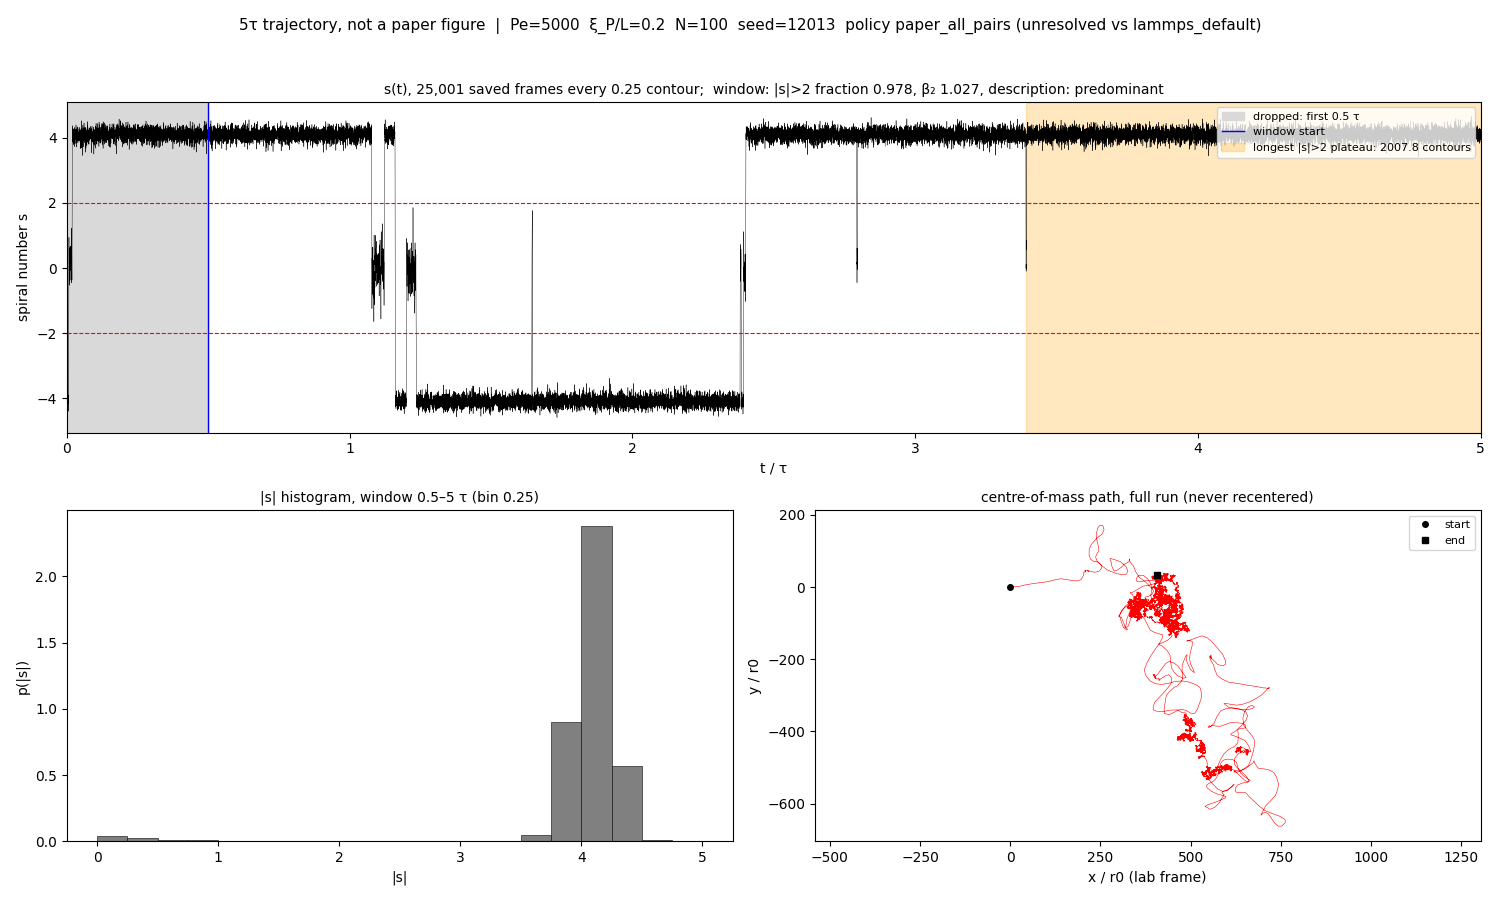
\includegraphics[width=\linewidth]{result_panel.png}
\caption{The finished $5\tau$ run. Top: the spiral number over time; grey is the start-up period we ignore, orange the longest unbroken spiral. Bottom left: how often each $|\spn|$ value occurred. Bottom right: the path of the centre of mass.}
\end{figure}

\begin{center}
\begin{tabular}{p{0.38\linewidth}p{0.18\linewidth}p{0.36\linewidth}}\toprule
measured (after the first $0.5\tau$) & value & meaning\\ \midrule
time with $|\spn|>2$ & 97.8\% & almost always wound up\\
$\beta_2$ & 1.03 & two sharp peaks at $\pm4$: spiral-dominated\\
longest unbroken spiral & $\geq2007.75$ contours & still intact when the run ended\\
centre-of-mass MSD slope & 1.00 & while wound, it drifts randomly instead of travelling\\
rotation slope-1 region & none & so no $D_r$ is reported\\
\textbf{description} & \textbf{predominant} & fraction $>1/2$ and $\beta_2<2$\\ \bottomrule
\end{tabular}
\end{center}

\textbf{Reading the top panel.}
\begin{itemize}
\item A spiral forms almost immediately and holds at $\spn\approx+4$ until about $1.1\tau$.
\item It breaks up briefly, then re-forms the other way round ($\spn\approx-4$) until about $2.4\tau$.
\item It flips back to $+4$ and stays there to the end.
\item A few single-snapshot dips are visible.
\end{itemize}
So spirals here do break and re-form; they are not permanent.

\textbf{Reading the histogram.} 97.7\% of snapshots have $|\spn|$ between 3.5 and 4.75, and only about 2\% are below 1. A tiny peak for ``stretched out'' and a huge peak for ``wound'' is the shape the paper describes for its strong-spiral example.

\textbf{Reading the path.} Dense tangles appear where the spiral spun in place and drifted randomly, linked by long straight stretches where the filament was unwound and crawling. The paper's Figure~2 caption describes exactly these ``separated clusters''.

\begin{figure}[H]\centering
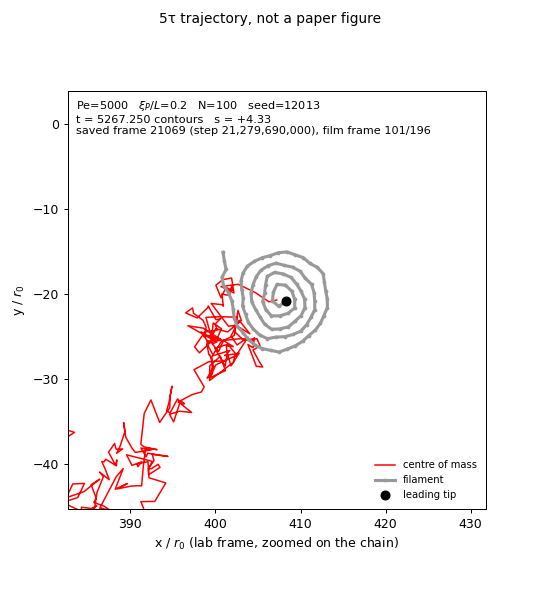
\includegraphics[width=0.42\linewidth]{frame_result_plateau.png}
\caption{A frame from the film of the longest spiral: four tight turns, head at the centre. The view follows the filament as it drifts.}
\end{figure}

%=====================================================================
\section{Is this a reproduction of the paper? Not yet}
%=====================================================================
\begin{warnbox}[title=Why ``agrees with the paper'' is not the same as ``reproduced the paper'']
\begin{itemize}
\item \textbf{One random seed.} Another seed (12003) did not even wind up in the first 10 contours. We do not know how typical our run is.
\item \textbf{One of three settings.} The polymer ($\Pe=200$) and weak-spiral ($\Pe=1000$) runs at full length have not been done.
\item \textbf{Unknown inputs.} The timestep and the repulsion setting are not published. Both could shift break-up rates.
\item \textbf{No numbers compared yet.} We compared shapes and descriptions, not values read off the paper's plots.
\item \textbf{Most figures untouched.} The motion figures (6, 8, 9, 10) and the phase diagram (Figure 4e) have not been computed at full length.
\end{itemize}
\end{warnbox}
In the project's six-stage ladder:
\begin{enumerate}
\item force law: done;
\item measuring tools: done;
\item spiral formation: partly done;
\item one long strong-spiral run: done, for one seed;
\item the other settings and the motion figures: not started;
\item the phase diagram: blocked on the missing inputs.
\end{enumerate}

%=====================================================================
\section{A tour of the code}
%=====================================================================
Everything lives in the folder \code{spin-chain-paper-v2/spin-chain-paper-v2}. The simulator is the Python package \code{src/spinchain}; the heavy number-crunching is compiled to machine code by \emph{Numba}.

\begin{figure}[H]\centering
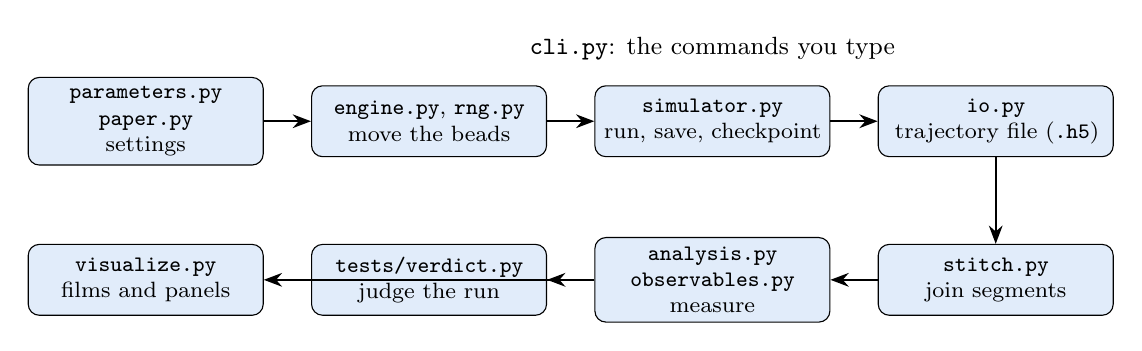
\begin{tikzpicture}[node distance=0.55cm and 0.6cm,box/.style={draw,rounded corners,fill=boxblue,align=center,font=\footnotesize,minimum height=0.9cm,text width=2.75cm},arr/.style={-{Stealth},thick}]
\node[box] (par) {\code{parameters.py}\\ \code{paper.py}\\ settings};
\node[box,right=of par] (eng) {\code{engine.py}, \code{rng.py}\\ move the beads};
\node[box,right=of eng] (sim) {\code{simulator.py}\\ run, save, checkpoint};
\node[box,right=of sim] (h5) {\code{io.py}\\ trajectory file (\code{.h5})};
\node[box,below=1.1cm of h5] (st) {\code{stitch.py}\\ join segments};
\node[box,left=of st] (an) {\code{analysis.py}\\ \code{observables.py}\\ measure};
\node[box,left=of an] (vd) {\code{tests/verdict.py}\\ judge the run};
\node[box,left=of vd] (vz) {\code{visualize.py}\\ films and panels};
\draw[arr] (par)--(eng); \draw[arr] (eng)--(sim); \draw[arr] (sim)--(h5); \draw[arr] (h5)--(st); \draw[arr] (st)--(an); \draw[arr] (an)--(vd); \draw[arr] (an)--(vz);
\node[above=0.2cm of sim,font=\small] {\code{cli.py}: the commands you type};
\end{tikzpicture}
\caption{How data flows through the code: settings, simulation, file, then stitching, measurement, verdict and pictures.}
\end{figure}

\begin{longtable}{p{0.27\linewidth}p{0.66\linewidth}}\toprule file & in plain words\\ \midrule\endhead
\code{parameters.py} & Turns $\Pe$ and $\xiP/L$ into actual forces and stiffness, refuses unsafe timesteps, and makes a fingerprint of the settings so files cannot be mixed up.\\
\code{paper.py} & The three Figure-2 settings (polymer, weak, strong) and their default seeds.\\
\code{rng.py} & The replayable random-number generator.\\
\code{forces.py} & A slow but simple force calculation used to check the fast one.\\
\code{engine.py} & The fast stepping routine with the neighbour list. (The old zero-reset is off and can only be switched on with bookkeeping.)\\
\code{simulator.py} & The loop: step, save a snapshot, flush, checkpoint, track the end-to-end angle.\\
\code{io.py} & Writes the trajectory file and labels it (origin, policy, timestep status).\\
\code{checkpoint.py} & Saves and reloads the exact state; refuses a checkpoint from different settings.\\
\code{observables.py} & The measuring tools: spiral number, kurtosis, MSDs, rotation, structure factor, plateau finder.\\
\code{analysis.py} & Reads a file and computes the paper's quantities over a window you choose.\\
\code{stitch.py} & Joins segments, refusing gaps, overlaps or mismatched starts.\\
\code{visualize.py} & Films and panels from saved snapshots only.\\
\code{cli.py} & The commands: \code{benchmark}, \code{headless}, \code{paper-reproduce}, \code{analyze}, \code{visualize}, and more.\\
\code{tests/} & 64 automatic tests, plus helper scripts: \code{smoke_integrity.py}, \code{formation_gate.py}, \code{verdict.py}, \code{result_figures.py}.\\
\code{output/} & Everything the runs produced: gate runs, films, the long run, verdict, figures.\\
\code{*.md} notes & One note per session, from \code{REPRO_NOTE.md} to \code{RESULT_NOTE.md}.\\ \bottomrule
\end{longtable}

\textbf{What is inside a trajectory file?}
\begin{itemize}
\item One row per saved snapshot: the step number, the time (in simulation units and in $\tau$), $\spn$, the centre of mass, the end-to-end vector and its counted-turns angle, the size of the coil, and all 101 bead positions.
\item Labels saying where the origin is, which end leads, which policy was used, and that the timestep is unpublished.
\item A ``complete'' flag that is true only if the run reached its target.
\end{itemize}

%=====================================================================
\section{How to run it yourself}
%=====================================================================
\subsection{One-time setup (Windows)}
Open a terminal in the folder \texttt{spin-chain-paper-v2\textbackslash spin-chain-paper-v2} and type:
\begin{lstlisting}[style=sh]
uv venv -p 3.11 .venv311
uv pip install -p .venv311/Scripts/python.exe -r requirements.txt
set PYTHONPATH=src
.venv311\Scripts\python.exe -m pytest -q
\end{lstlisting}
The last line should end with ``64 passed''. (\code{uv} is a fast Python installer. With ordinary Python, create a 3.11 environment and run \code{pip install -r requirements.txt}.)
In every new terminal, run \code{set PYTHONPATH=src} again, or use the full commands below.

\subsection{Recipe 1: how fast is my computer?}
\begin{lstlisting}[style=sh]
.venv311\Scripts\python.exe -m spinchain benchmark --regime strong_spiral --policy paper_all_pairs --steps 20000
\end{lstlisting}
Read \code{steps_per_second}. Then $2.525\times10^{10}$ divided by that number gives the seconds for a $5\tau$ run.

\subsection{Recipe 2: a quick look (minutes)}
\begin{lstlisting}[style=sh]
.venv311\Scripts\python.exe -m spinchain headless --regime strong_spiral --steps 2000000 --sample-every 10000 --output output/viz/try.h5 --overwrite
.venv311\Scripts\python.exe -m spinchain visualize output/viz/try.h5
\end{lstlisting}
This writes \code{output/viz/try.gif} (a film) and \code{try.png} (a panel). It is far too short for spirals; it is just a look.

\subsection{Recipe 3: the formation gate (about 5 minutes per run)}
\begin{lstlisting}[style=sh]
.venv311\Scripts\python.exe -m spinchain headless --regime strong_spiral --policy paper_all_pairs --steps 40400000 --sample-every 101000 --output output/gate/my-gate.h5 --overwrite
.venv311\Scripts\python.exe tests/formation_gate.py --name mygate output/gate/my-gate.h5
\end{lstlisting}
Ten contours at $\Pe=5000$ is 40\,400\,000 steps. The script prints whether the gate passed and draws \code{mygate_s_t.png}.

\subsection{Recipe 4: a full $5\tau$ run (about 2.5 days)}
\begin{warnbox}[title=Start long runs yourself]
Start long runs from your own terminal or by double-clicking a script, \emph{not} from inside the AI assistant. A job started by the app can be killed when the app updates, which is exactly what happened to us. Keep the window open, keep the laptop plugged in, and use the ``Best performance'' power mode.
\end{warnbox}
\begin{lstlisting}[style=sh]
.venv311\Scripts\python.exe -m spinchain paper-reproduce --regime strong_spiral --policy paper_all_pairs --seed 12013 --tau 5 --replicates 1 --output-dir output/reproduction/my-run --i-know
\end{lstlisting}
\begin{itemize}
\item \textbf{Watch progress} by looking at the last lines of the log (\code{progress: step=... tau=...}). Do \emph{not} open the \code{.h5} file while it is being written.
\item \textbf{If it stops,} run the same command with \code{--resume} added. It picks up from the last checkpoint and writes a new segment file.
\item \textbf{It is finished} when the log ends with \code{"completed": true}.
\end{itemize}

\subsection{Recipe 5: stitch, judge, draw}
\begin{lstlisting}[style=sh]
.venv311\Scripts\python.exe -c "import glob;from spinchain.stitch import write_stitched;print(write_stitched(glob.glob('output/reproduction/my-run/strong_spiral-seed12013*.h5'),'output/reproduction/my-run-stitched.h5'))"
.venv311\Scripts\python.exe tests/verdict.py output/reproduction/my-run-stitched.h5 --out output/reproduction/my-verdict.json
.venv311\Scripts\python.exe tests/result_figures.py output/reproduction/my-run-stitched.h5 output/reproduction/my-verdict.json --out-dir output/reproduction/my-result
\end{lstlisting}

\subsection{Common problems}
\begin{description}[style=nextline]
\item[``FileExistsError''] The output file already exists. Choose a new name. Add \code{--overwrite} only if you really want to throw the old one away.
\item[``fingerprint mismatch''] You are resuming with different settings (seed, policy, $\Pe$) from the original run.
\item[The verdict says ``refused''] The run is shorter than $5\tau$, or the file is damaged or unlabelled. The message says which.
\item[A path like \code{/c/Users} creates odd folders] In Windows Python, write \code{C:/Users/...}.
\item[It is slow] Plug in, use Best performance, close heavy programs. Spiral phases run a little slower because more beads touch.
\end{description}

%=====================================================================
\section{Where to go next, and why}
%=====================================================================
\begin{enumerate}
\item \textbf{Find the missing numbers (hours).}
\begin{itemize}
\item Download the paper's supplementary file; it may list the timesteps and the simulation input.
\item Measure numbers off the paper's plots (``digitize'' them), so we can compare values, not just shapes.
\end{itemize}
\item \textbf{Run several jobs at once (about 3 days).} The laptop has 8 logical cores and each job uses one, so run together:
\begin{itemize}
\item $\Pe=200$ and $\Pe=1000$, to see all three regimes;
\item seed 12003 and one new seed at $\Pe=5000$, to test how typical our result is;
\item seed 12013 under the other policy, to see whether break-ups differ.
\end{itemize}
\item \textbf{The motion figures (6, 8, 9, 10).} These need other settings and, for Figure~6, snapshots close together.
\item \textbf{The phase diagram.} About 100--150 days of single-core computing: a project for a computing cluster, or for one slice of the diagram.
\end{enumerate}

%=====================================================================
\section{Glossary}
%=====================================================================
\begin{description}[style=nextline,itemsep=0.1em]
\item[Bead--spring model] A filament represented as beads joined by springs.
\item[Brownian motion] Random jiggling caused by molecular collisions.
\item[Checkpoint] A saved exact state from which a run can continue.
\item[Contour time] Time for the filament to crawl one body length; 202 time units at $\Pe=5000$.
\item[Euler--Maruyama] The simplest correct step rule for equations with random noise.
\item[Excluded volume (WCA)] Short-range repulsion that prevents the filament crossing itself.
\item[Flexure number $\Flex$] Pushing versus stiffness; large values favour spirals.
\item[Gate] A cheap pre-test run before an expensive one.
\item[$\kT$] Thermal energy, the unit of energy here.
\item[Kurtosis $\beta_2$] A shape number: 3 for a bell curve, 1 for two sharp peaks.
\item[MSD] Mean square displacement: average squared distance moved over a time lag.
\item[Neighbour (Verlet) list] A saved list of nearby bead pairs, rebuilt only when needed.
\item[Overdamped] Friction dominates inertia: velocity is proportional to force.
\item[Péclet number] Directed motion versus diffusion.
\item[Persistence length $\xiP$] The distance over which the filament keeps its direction.
\item[Plateau] A stretch of consecutive snapshots with $|\spn|>2$.
\item[Policy] Which nearby bead pairs feel the repulsion. Unresolved, because the setting is unpublished.
\item[Railway motion] The filament sliding along its own outline.
\item[Seed] The integer that determines the whole stream of random numbers.
\item[Segment] One file of a run that was interrupted and resumed.
\item[Spiral number $\spn$] Total turning along the filament, in full turns.
\item[Stitching] Joining segments into one exact trajectory.
\item[$\tau$] The time to diffuse one's own length; $5\tau$ is the paper's run length.
\item[Verdict] Pre-written rules that describe a finished run.
\end{description}

%=====================================================================
\section{Exercises (answers below)}
%=====================================================================
\begin{enumerate}
\item With $L=100$, $\kT=1$: what is $f_p$ for $\Pe=1000$? What is the flexure number at $\xiP/L=0.2$?
\item How many steps is $5\tau$ at $\Delta t=5\times10^{-5}$, with $\tau=252\,500$? How long at 120\,000 steps/s?
\item A filament's $|\spn|$ is exactly 4 half the time and exactly 0 the other half. What is the symmetrized $\beta_2$?
\item Why does resetting the centre of mass to zero in every saved frame ruin the centre-of-mass MSD, but not the spiral number?
\item Two runs use the same seed but different policies. Why can their spiral histories look almost identical?
\item The verdict saw fraction $=0.3$ and a 5-contour plateau. Which description applies?
\item Why must the random numbers depend on (seed, step, bead) and not on ``how many numbers were drawn so far''?
\item Paper bead 25 is which code bead for $N=100$? Why is there a difference?
\end{enumerate}

\subsection*{Answers}
\begin{enumerate}
\item $f_p=1000/100^2=0.1$; $\Flex=1000/0.2=5000$.
\item $5\times252\,500/(5\times10^{-5})=2.525\times10^{10}$ steps; divided by $1.2\times10^5$ steps/s gives $2.1\times10^5$\,s, about 58 hours.
\item Values $\{\pm4,\pm4,0,0\}$ in equal proportion: the mean is 0, the variance is 8, the fourth moment is $128$, so $\beta_2=128/64=2$.
\item The MSD compares positions at different times. If every frame is shifted back to the origin, the measured displacement is only the noise inside one reset period. The spiral number depends only on the shape within a single frame, which a shift does not change.
\item Same seed means identical random kicks. The policies differ only for beads at most 3 apart, while spirals form when far-apart beads touch.
\item \emph{Intermittent}: a plateau longer than 2 contours exists and the fraction is below 1/2.
\item So a run that is split, stopped and resumed draws exactly the same numbers and reproduces the same trajectory bit for bit.
\item Code bead $101-25=76$. The paper's propulsion pushes towards bead 1 and ours towards the last bead: the same physics, numbered backwards.
\end{enumerate}

\appendix
\section{Key numbers}
\begin{center}\small
\begin{tabular}{lp{0.6\linewidth}}\toprule
beads / bonds & 101 / 100\\
$\kappa$, $k_S$, $\Delta t$ & 20, 4000, $5\times10^{-5}$ (timestep unpublished)\\
$\tau$ & 252\,500 time units ($5.05\times10^9$ steps)\\
contour time at $\Pe=5000$ & 202 time units ($4.04\times10^6$ steps)\\
long run & seed 12013, \code{paper_all_pairs}, $5\tau$, 25\,001 snapshots, about 55 h of computing\\
result & 97.8\% of the time $|\spn|>2$; $\beta_2=1.03$; longest spiral $\geq2007.75$ contours; \emph{predominant}\\ \bottomrule
\end{tabular}
\end{center}

\section{How these reports were built}
Both reports are \LaTeX{} documents in the folder \code{reports/}. The expert report is in \code{expert/} and this one in \code{beginner/}; they share the preamble \code{common/preamble.tex} and the folder \code{figures/}.
To rebuild one, run \code{pdflatex report_beginner.tex} twice in its folder. The second pass fills in the table of contents and cross-references.

\vspace{1em}
\begin{keybox}
\textbf{Take-home message.} We now have a simulator we trust, tools that measure what the paper measures, and one long run in which the filament was spiral-wound almost all the time.
That matches the paper's strong-spiral picture \emph{for this run}. To call it a reproduction, we need more seeds, the other settings, and the unpublished inputs.
\end{keybox}

\end{document}
